\documentclass[DIV13,a4paper]{scrartcl}

\usepackage[T1]{fontenc}
\usepackage[utf8]{inputenc}
\usepackage[english]{babel}

\usepackage[default,scale=0.95]{opensans}
\usepackage[scaled=0.85]{beramono}


\usepackage{listings}
\usepackage{tabularx}
\usepackage{booktabs}
\usepackage{grid-system}
\usepackage{graphicx}
\usepackage{multirow} % Required for multirows
\usepackage{bbding}
\usepackage{wrapfig}

\usepackage{xcolor}
\definecolor{linkcolor}{rgb}{0, 0, 0.93}

\usepackage[
hidelinks,
colorlinks=true,
urlcolor=linkcolor
]{hyperref}


\setlength{\parindent}{0cm}
\lstset{language=[LaTeX]tex,xleftmargin=2em}

\title{Grid System}
\author{Marcus Bitzl\\ \url{marcus@bitzl.com}}

\begin{document}
	\maketitle
	
	\begin{abstract}
		Grid system is a package that implements grid like layouts for \LaTeX, as it is commonly known from CSS. You can easily divide your horizontal space into equal parts and assign these to boxes containing your content.
	\end{abstract}
	
	\section{Usage}
	There are two environments to divide your area into boxes: \texttt{row} to divide your area into columns and \texttt{cell} to fill the area with content:
	
	\medskip
	
	\begin{lstlisting}
\begin{row}{<Number of columns}{<Number of cells>}
	\begin{cell}{<Number of columns to span>}
		...
	\end{cell}
	\begin{cell}{<Number of columns to span>}
		...
	\end{cell}
\end{row}
	\end{lstlisting}
	
	Each cell is created using a \texttt{minipage} environment. In future versions the will be a switch to choose either minipages or parboxes.
	
	\section{Parameters}
	There is one optional parameter for the environment \texttt{row} right now:
	
	\medskip
	
	\begin{tabularx}{\linewidth}{llX}\toprule
		\textbf{Parameter} & \textbf{Default} & \textbf{Description},\\ \midrule 
		cellsep & 1.75em & horizonal space between two cells.\\\bottomrule
	\end{tabularx}
	
	\section{Contribute}
	You want to contribute? Just fork me on Github, start discussions and send me you pull requests: 
	\begin{center}
		\href{https://github.com/bitzl/latex-grid-system}{\ttfamily bitzl/latex-grid-system}
	\end{center}
	
	
	
	\section{License}
	Copyright 2013 Marcus Bitzl
	
	\medskip
	
	Licensed under the Apache License, Version 2.0 (the "License");
	you may not use this file except in compliance with the License.
	You may obtain a copy of the License at
	
	\medskip
	
	\hspace*{1.2em}\href{http://www.apache.org/licenses/LICENSE-2.0}{\texttt{http://www.apache.org/licenses/LICENSE-2.0}}
	
	\medskip
	
	Unless required by applicable law or agreed to in writing, software
	distributed under the License is distributed on an "AS IS" BASIS,
	WITHOUT WARRANTIES OR CONDITIONS OF ANY KIND, either express or implied.
	See the License for the specific language governing permissions and
	limitations under the License.
	
	
	\section{Example}
	\begin{row}[cellsep=0.75cm]{3}{3}
		\begin{cell}{1}
			\section*{Overview}
			\vspace{-1.5ex}
			This shows what you can do with the \texttt{grid-system} package and three columns.
		\end{cell}
		\begin{cell}{1}
			\section*{Why use it?}
			\vspace{-1.5ex}
			Sometimes you need to split your text in several independent columns based on equal division of the available space. This package allows you to easily do so.
		\end{cell}
		\begin{cell}{1}
			\section*{Contribute}
			\vspace{-1.5ex}
			You want to contribute? Just fork me on Github, start discussions and send me you pull requests: 
			\begin{center}
				\href{https://github.com/bitzl/latex-grid-system}{\ttfamily bitzl/latex-grid-system}
			\end{center}
		\end{cell}
	\end{row}
	
	\bigskip
	
	\begin{row}[cellsep=0.75cm]{3}{2}
		\begin{cell}{2}
			\section*{License}
			\vspace{-1.5ex}
			Copyright 2013 Marcus Bitzl
			
			\medskip
			
			Licensed under the Apache License, Version 2.0 (the "License");
			you may not use this file except in compliance with the License.
			You may obtain a copy of the License at
			
			\medskip
			
			\hspace*{1.2em}\href{http://www.apache.org/licenses/LICENSE-2.0}{\texttt{http://www.apache.org/licenses/LICENSE-2.0}}
			
			\medskip
			
			Unless required by applicable law or agreed to in writing, software
			distributed under the License is distributed on an "AS IS" BASIS,
			WITHOUT WARRANTIES OR CONDITIONS OF ANY KIND, either express or implied.
			See the License for the specific language governing permissions and
			limitations under the License.
		\end{cell}%
		\begin{cell}{1}
			\section*{Why use it?}
			\vspace{-1.5ex}
			Sometimes you need to split your text in several independent columns based on equal division of the available space. This package allows you to easily do so.
		\end{cell}
	\end{row}
	
	\bigskip
	
	\begin{row}[cellsep=0.75cm]{3}{2}
		\begin{cell}{1}
			\section*{Short}
			\vspace{-1.5ex}
			This shows the capabilities of grid-system with three equal columns.
		\end{cell}
		\begin{cell}{2}
			\section*{Long}
			\vspace{-1.5ex}
			Sometimes you need to split your text in several independent columns based on equal division of the available space. This package allows you to easily do so.
		\end{cell}
	\end{row}
	
	\clearpage
	
	\section{minipage}
	\begin{figure}[!h]
		\vspace{0.3cm}
		\begin{center}
			\begin{minipage}{0.49\linewidth}
				\centerline{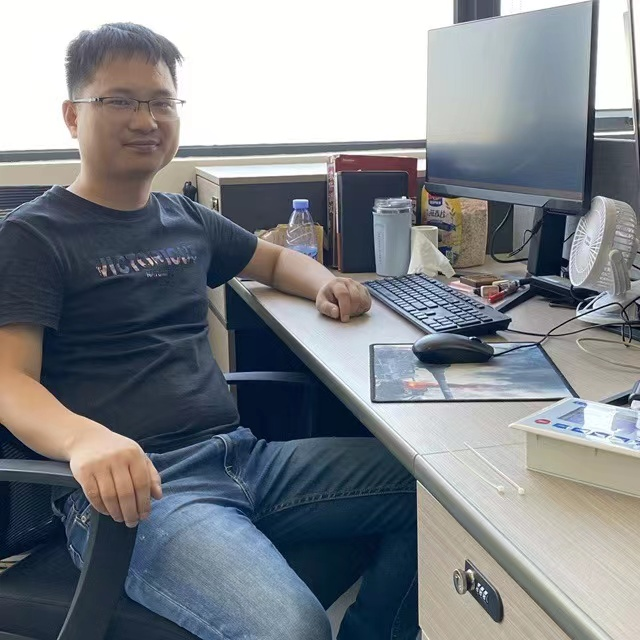
\includegraphics[width=1\linewidth]{ShowMe.jpg}}
			\end{minipage}
			\hfill
			\begin{minipage}{0.49\linewidth}
				\centerline{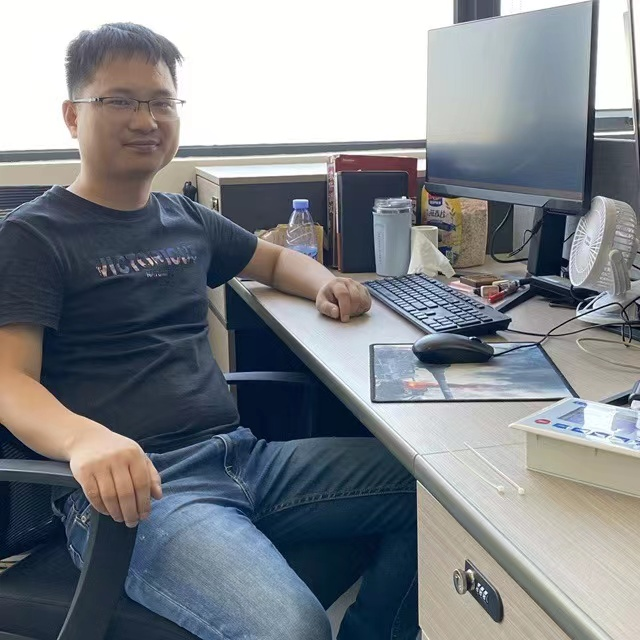
\includegraphics[width=1\linewidth]{ShowMe}}
			\end{minipage}
			\vfill
			\vspace{0.2cm}
			\begin{minipage}{0.49\linewidth}
				\small
				\centerline{(aaaaa)}
			\end{minipage}
			\hfill
			\begin{minipage}{0.49\linewidth}
				\small
				\centerline{(bbbbb)}
			\end{minipage}
		\end{center}
		\caption{t-SNE visualization of the distribution of (a) representations and (b) maps. }
		\vspace{0.3cm}
		\label{fig_tsne}
	\end{figure}
	\begin{minipage}[c]{0.5\textwidth}
	\centering
	\label{tab:ablation2}
	\setlength{\tabcolsep}{0.5 mm}
	\scalebox{0.9}{
		\begin{tabular}{c|cc|cc|cc}
			\hline
			\multirow{2}*{p}  & \multicolumn{2}{c|}{Stage I } &    \multicolumn{2}{c|}{Stage II}  \\
			&PSNR   &   LPIPS   &PSNR   &   LPIPS   &   $\Delta$PSNR    &   $\Delta$LPIPS
			\\
			\hline
			8   &  35.00    &	0.0000	&    20.00	& 0.0000 &-10.00 &   0.0000  \\
			16   &  35.00    &	0.0000	&    20.00	& 0.0000 &-10.00 &   0.0000  \\
			32   &  35.00    &	0.0000	&    20.00	& 0.0000 &-10.00 &   0.0000  \\
			64   &  35.00    &	0.0000	&    20.00	& 0.0000 &-10.00 &   0.0000  \\
			\hline
		\end{tabular}
	}
	\captionof{table}{Ablation studies 1.}
	\end{minipage}
	\begin{minipage}[c]{0.5\textwidth}
		\centering
		\label{tab:ablation}
		\setlength{\tabcolsep}{0.5mm}
		\vspace{-1mm}
		\scalebox{0.85}{
			\begin{tabular}{lcc|cccc}
				\hline
				MMM  &    PPP &   AAA &  PSNR$\uparrow$    &   LPIPS$\downarrow$ & VOI-S$\downarrow$    &   VOI-M$\downarrow$
				\\
				\hline
				\XSolidBrush   & \XSolidBrush & \XSolidBrush& 23.00  & 0.5000  &   4.0000    &   2.0000 \\
				\XSolidBrush   &  \Checkmark  & \Checkmark & 23.00  & 0.5000  &   4.0000    &   2.0000 \\
				\Checkmark & \XSolidBrush  & \Checkmark    & 23.00  & 0.5000  &   4.0000    &   2.0000 \\
				\Checkmark  & \Checkmark   & \XSolidBrush  & 23.00  & 0.5000  &   4.0000    &   2.0000 \\
				\Checkmark  & \Checkmark   & \Checkmark   & 23.00  & 0.5000  &   4.0000    &   2.0000 \\
				\hline
			\end{tabular}
		}
		\captionof{table}{Ablation studies 2.}
	\end{minipage}
	
	\clearpage
	
	\section{float layout}
	\begin{minipage}[c]{0.7\textwidth}
		  Here is a bunch of text that we can put around an image.  The image will be shown on the left
		side of the paper, but our text can go all around it.  There will be spacing above and below the
		image where text can go.  This spacing can actually be controlled by using a negative value with
		\texttt{vskip}, but we will not be going into that here.  It will be just our little secret: you,
		me, and the compiler.  I hope this is enough dummy text for this example.  If not, I will have to
		type up some more.
		\begin{wrapfigure}{l}{0.60\textwidth}
			\centering
			
\includegraphics[width=0.78\textwidth]{lion.png}
		\end{wrapfigure}
		Oops, I just tried compiling it.  Apparently I need to include a bit more.  I could go on a bit
		and tell you more secrets of image placement.  Did you know that you can use the \texttt{center}
		environment around the \texttt{includeimage} to make things look even prettier?  It's true.  The
		control which \LaTeX provides with it is nice.
	\end{minipage}
\end{document}